\section{Равновесие текучей среды}
\begin{align*}
  &\frac{d\rho}{dt} = -\rho(\nabla \cdot \vec{V}) \\
  &\rho \frac{d \vec{V}}{dt} = \nabla \cdot \overleftrightarrow{P} + \rho \vec{f} \\
  & \rho \frac{d E}{dt} = \overleftrightarrow{P} \cdot \vec{S} - \nabla \cdot \vec{q} + \rho Q \\
  &\rho(\vec{r}. t),\ \vec{V}(\vec{r}, t), E(\vec{r}, t) \\
  &\overleftrightarrow{P} = \overleftrightarrow{P} (\overleftrightarrow{S}),\ \vec{q} = \vec{q}(E)
\end{align*}

\begin{defn}
  Текучая среда --- среда, которая приходит в движение под действием сколь
  угодно малого касательного напряжения.
\end{defn}

\begin{figure}[h]
    \centering
    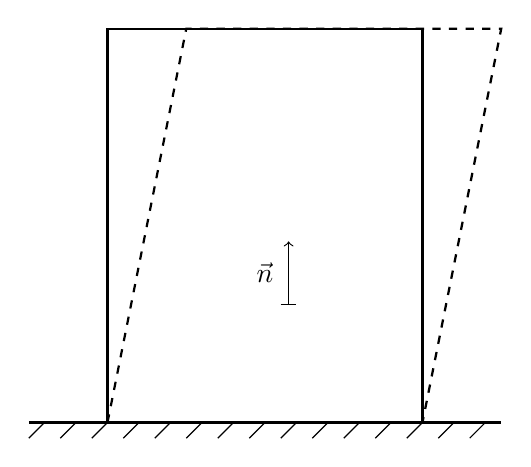
\begin{tikzpicture}
    \draw[thick] (-3, 0) -- (3, 0); % основание
    \draw[thick] (-2, 0) coordinate (A) -- (-2, 5) -- (2, 5) -- (2, 0) coordinate (B);
    \draw[thick,dashed] (A) -- (-1, 5) -- (3, 5) -- (B);
    \foreach \x in {-2.8, -2.4, ..., 3 } {
        \draw (\x, 0) -- ++(-0.2, -0.2);
    }
    \node at (0, 1.9) {$\vec n$};
    \draw [arrows=->] (0.3, 1.5) -- (0.3, 2.3);
    \draw (0.2, 1.5) -- (0.4, 1.5);
\end{tikzpicture}

    \caption{Напряжения в твёрдом теле}
\end{figure}

\begin{note}
  Если среда находится в состоянии покая, значит в ней нет касательных напряжений.
\end{note}

*pic2*
\[
  \vec{P}_n = P_n \vec(n)
\]

\begin{align*}
  &\vec{P}_1 = P_{11} \vec{e}_1 \\
  &\vec{P}_2 = P_{22} \vec{e}_2 \\
  &\vec{P}_3 = P_{33} \vec{e}_3 \\
\end{align*}

\[
  P_{ij} = \begin{cases}
    0, \quad i \neq j \\
    P_{ii}, \quad i = j
  \end{cases}
\]

\[
  \overleftrightarrow{P} =
  \begin{pmatrix}
    p_{11} &0 &0 \\
    0 &p_{22} &0 \\
    0 &0 &p_{33}
  \end{pmatrix}
\]

\begin{note}[Формула Коши]
  \begin{align*}
    &\vec{p}_n = \overleftrightarrow{P} \cdot \vec{n} \\
    &p_n \begin{pmatrix}
        n_1 \\
        n_2 \\
        n_3
      \end{pmatrix} = \begin{pmatrix} p_{11} &0 &0 \\
        0 &p_{22} &0 \\
        0 &0 &p_{33}
    \end{pmatrix} \cdot
               \begin{pmatrix}
                 n_1 \\
                 n_2 \\
                 n_3
               \end{pmatrix}
  \end{align*}
\[
p_n = p_{11} = p_{22} = p_{33} = \underbrace{-p}_{\text{давление}}
\]
\end{note}

\[
\overleftrightarrow{P} =
\begin{pmatrix}
  -p &0 &0\\
  0 &-p &0\\
  0 &0 &-p
\end{pmatrix} = -p
\begin{pmatrix}
  1 &0 &0 \\
  0 &1 &0 \\
  0 &0 &1
\end{pmatrix} = -p \cdot \overleftrightarrow{E}
\]

\begin{note}[Закон Паскаля]
  При равновесии текучей среды нормальное напряжение на произвольно выбранной
  площадке не зависит от ее ориентации.
\end{note}

Уравнение переноса импульса.
\begin{align*}
  & \rho \frac{d\vec{V}}{dt} = \nabla \cdot \overleftrightarrow{P} + \rho \cdot \vec{f} \\
  & \nabla \cdot \overleftrightarrow{P} = \begin{pmatrix}
      \frac{\partial}{\partial x_1} & \frac{\partial}{\partial x_2} & \frac{\partial}{\partial x_3}
    \end{pmatrix} \cdot \begin{pmatrix}
      -p &0 &0 \\
      0 &-p &0 \\
      0 &0 &-p
    \end{pmatrix} = \begin{pmatrix}
      -\frac{\partial p}{\partial x_1} & -\frac{\partial p}{\partial x_2} & -\frac{\partial p}{\partial x_3}
    \end{pmatrix} = \underbrace{-\nabla p}_{\text{градиент}}\\
  &\nabla \cdot \overleftrightarrow{P}= - \nabla P \\
  &\frac 1\rho \nabla p = \vec{f} \text{ --- Уравнение Эйлера равновесия текучей среды}
\end{align*}

\begin{defn}
  $\rho = \rho(p)$ --- \textbf{баротропность}.
\end{defn}

\begin{align*}
  &p V = \frac{R}{\mu} M T \\
  &p \,dV = \frac{R}{\mu} \,dm\, T\\
  &p = \frac{R}{\mu} \rho T \\
  &\rho  = \frac{p \mu}{RT}
\end{align*}

Изотермический процесс.
\[
  T = T_0,\ \rho = \frac{p \mu}{R T_0} = cp
\]

Адиабатический процесс.
\[
  \rho = c p^{-\frac{1}{\gamma}},\ \gamma = \frac{c_p}{c_\rho}
\]

\begin{defn}
  \begin{align*}
    &\P(p) = \int_{p_0}^p \frac{dp}{\rho(p)} \text{ --- потенциал давления} \\
    &\frac{\partial \P}{\partial x_1} = \frac{d \P}{d p} \frac{\partial p}{\partial x_1}= \frac{1}{\rho} \frac{\partial p}{\partial x_1} \\
    & \nabla \P = \frac{1}{\rho} \nabla p
  \end{align*}
\end{defn}

\begin{align*}
  &\nabla \times \vec{f} = 0 \\
  &\vec{f} = -\nabla \Pi \\
  &\nabla \P = \nabla \Pi \\
  &\nabla (\P + \Pi)= 0 \\
  &\P + \Pi = const
\end{align*}

\begin{note}
  При баротропном равновесии текучей среды в потенциальном поле сил сумма
  потенциала давления и потенциала силы не меняется.
\end{note}

\begin{cor}
  \[
    \Pi = const \implies \P = const  \implies
    \begin{cases}
      p = const \\
      \rho = cosnt \\
      T = const
    \end{cases}
  \]
\end{cor}


